%%%%%%%%%%%%%%%%%%%%%%%%%%%%%%%%%%%%%%%%
% datoteka diploma-vzorec.tex
%
% vzorčna datoteka za pisanje diplomskega dela v formatu LaTeX
% na UL Fakulteti za računalništvo in informatiko
%
% vkup spravil Gašper Fijavž, december 2010
% 
%
%
% verzija 12. februar 2014 (besedilo teme, seznam kratic, popravki Gašper Fijavž)
% verzija 10. marec 2014 (redakcijski popravki Zoran Bosnić)
% verzija 11. marec 2014 (redakcijski popravki Gašper Fijavž)
% verzija 15. april 2014 (pdf/a 1b compliance, not really - just claiming, Damjan Cvetan, Gašper Fijavž)
% verzija 23. april 2014 (privzeto cc licenca)
% verzija 16. september 2014 (odmiki strain od roba)
% verzija 28. oktober 2014 (odstranil vpisno številko)
% verija 5. februar 2015 (Literatura v kazalu, online literatura)
% verzija 25. september 2015 (angl. naslov v izjavi o avtorstvu)
% verzija 26. februar 2016 (UL izjava o avtorstvu)
% verzija 16. april 2016 (odstranjena izjava o avtorstvu)
% verzija 5. junij 2016 (Franc Solina dodal vrstice, ki jih je označil s svojim imenom)


\documentclass[a4paper, 12pt]{book}

\usepackage[utf8x]{inputenc}   % omogoča uporabo slovenskih črk kodiranih v formatu UTF-8
\usepackage[slovene,english]{babel}    % naloži, med drugim, slovenske delilne vzorce
\usepackage[pdftex]{graphicx}  % omogoča vlaganje slik različnih formatov
\usepackage{fancyhdr}          % poskrbi, na primer, za glave strani
\usepackage{amssymb}           % dodatni simboli
\usepackage{amsmath}           % eqref, npr.
%\usepackage{hyperxmp}
\usepackage[hyphens]{url}  % dodal Solina
\usepackage{comment}       % dodal Solina

\usepackage[pdftex, colorlinks=true,
						citecolor=black, filecolor=black, 
						linkcolor=black, urlcolor=black,
						pagebackref=false, 
						pdfproducer={LaTeX}, pdfcreator={LaTeX}, hidelinks]{hyperref}

\usepackage{color}       % dodal Solina
\usepackage{soul}       % dodal Solina

%%%%%%%%%%%%%%%%%%%%%%%%%%%%%%%%%%%%%%%%
%	DIPLOMA INFO
%%%%%%%%%%%%%%%%%%%%%%%%%%%%%%%%%%%%%%%%
\newcommand{\ttitle}{Optimizacija strojne kode brez časovnih omejitev}
\newcommand{\ttitleEn}{Diploma thesis sample}
\newcommand{\tsubject}{\ttitle}
\newcommand{\tsubjectEn}{\ttitleEn}
\newcommand{\tauthor}{Franko Jančič}
\newcommand{\tkeywords}{računalnik, računalnik, računalnik}
\newcommand{\tkeywordsEn}{computer, computer, computer}


%%%%%%%%%%%%%%%%%%%%%%%%%%%%%%%%%%%%%%%%
%	HYPERREF SETUP
%%%%%%%%%%%%%%%%%%%%%%%%%%%%%%%%%%%%%%%%
\hypersetup{pdftitle={\ttitle}}
\hypersetup{pdfsubject=\ttitleEn}
\hypersetup{pdfauthor={\tauthor, matjaz.kralj@fri.uni-lj.si}}
\hypersetup{pdfkeywords=\tkeywordsEn}


 


%%%%%%%%%%%%%%%%%%%%%%%%%%%%%%%%%%%%%%%%
% postavitev strani
%%%%%%%%%%%%%%%%%%%%%%%%%%%%%%%%%%%%%%%%  

\addtolength{\marginparwidth}{-20pt} % robovi za tisk
\addtolength{\oddsidemargin}{40pt}
\addtolength{\evensidemargin}{-40pt}

\renewcommand{\baselinestretch}{1.3} % ustrezen razmik med vrsticami
\setlength{\headheight}{15pt}        % potreben prostor na vrhu
\renewcommand{\chaptermark}[1]%
{\markboth{\MakeUppercase{\thechapter.\ #1}}{}} \renewcommand{\sectionmark}[1]%
{\markright{\MakeUppercase{\thesection.\ #1}}} \renewcommand{\headrulewidth}{0.5pt} \renewcommand{\footrulewidth}{0pt}
\fancyhf{}
\fancyhead[LE,RO]{\sl \thepage} 
%\fancyhead[LO]{\sl \rightmark} \fancyhead[RE]{\sl \leftmark}
\fancyhead[RE]{\sc \tauthor}              % dodal Solina
\fancyhead[LO]{\sc Diplomska naloga}     % dodal Solina


\newcommand{\BibTeX}{{\sc Bib}\TeX}

%%%%%%%%%%%%%%%%%%%%%%%%%%%%%%%%%%%%%%%%
% naslovi
%%%%%%%%%%%%%%%%%%%%%%%%%%%%%%%%%%%%%%%%  


\newcommand{\autfont}{\Large}
\newcommand{\titfont}{\LARGE\bf}
\newcommand{\clearemptydoublepage}{\newpage{\pagestyle{empty}\cleardoublepage}}
\setcounter{tocdepth}{1}	      % globina kazala

%%%%%%%%%%%%%%%%%%%%%%%%%%%%%%%%%%%%%%%%
% konstrukti
%%%%%%%%%%%%%%%%%%%%%%%%%%%%%%%%%%%%%%%%  
\newtheorem{izrek}{Izrek}[chapter]
\newtheorem{trditev}{Trditev}[izrek]
\newenvironment{dokaz}{\emph{Dokaz.}\ }{\hspace{\fill}{$\Box$}}

%%%%%%%%%%%%%%%%%%%%%%%%%%%%%%%%%%%%%%%%%%%%%%%%%%%%%%%%%%%%%%%%%%%%%%%%%%%%%%%
%% PDF-A
%%%%%%%%%%%%%%%%%%%%%%%%%%%%%%%%%%%%%%%%%%%%%%%%%%%%%%%%%%%%%%%%%%%%%%%%%%%%%%%

%%%%%%%%%%%%%%%%%%%%%%%%%%%%%%%%%%%%%%%% 
% define medatata
%%%%%%%%%%%%%%%%%%%%%%%%%%%%%%%%%%%%%%%% 
\def\Title{\ttitle}
\def\Author{\tauthor, matjaz.kralj@fri.uni-lj.si}
\def\Subject{\ttitleEn}
\def\Keywords{\tkeywordsEn}

%%%%%%%%%%%%%%%%%%%%%%%%%%%%%%%%%%%%%%%% 
% \convertDate converts D:20080419103507+02'00' to 2008-04-19T10:35:07+02:00
%%%%%%%%%%%%%%%%%%%%%%%%%%%%%%%%%%%%%%%% 
\def\convertDate{%
    \getYear
}

{\catcode`\D=12
 \gdef\getYear D:#1#2#3#4{\edef\xYear{#1#2#3#4}\getMonth}
}
\def\getMonth#1#2{\edef\xMonth{#1#2}\getDay}
\def\getDay#1#2{\edef\xDay{#1#2}\getHour}
\def\getHour#1#2{\edef\xHour{#1#2}\getMin}
\def\getMin#1#2{\edef\xMin{#1#2}\getSec}
\def\getSec#1#2{\edef\xSec{#1#2}\getTZh}
\def\getTZh +#1#2{\edef\xTZh{#1#2}\getTZm}
\def\getTZm '#1#2'{%
    \edef\xTZm{#1#2}%
    \edef\convDate{\xYear-\xMonth-\xDay T\xHour:\xMin:\xSec+\xTZh:\xTZm}%
}

\expandafter\convertDate\pdfcreationdate 

%%%%%%%%%%%%%%%%%%%%%%%%%%%%%%%%%%%%%%%%
% get pdftex version string
%%%%%%%%%%%%%%%%%%%%%%%%%%%%%%%%%%%%%%%% 
\newcount\countA
\countA=\pdftexversion
\advance \countA by -100
\def\pdftexVersionStr{pdfTeX-1.\the\countA.\pdftexrevision}


%%%%%%%%%%%%%%%%%%%%%%%%%%%%%%%%%%%%%%%%
% XMP data
%%%%%%%%%%%%%%%%%%%%%%%%%%%%%%%%%%%%%%%%  
\usepackage{xmpincl}
\includexmp{pdfa-1b}

%%%%%%%%%%%%%%%%%%%%%%%%%%%%%%%%%%%%%%%%
% pdfInfo
%%%%%%%%%%%%%%%%%%%%%%%%%%%%%%%%%%%%%%%%  
\pdfinfo{%
    /Title    (\ttitle)
    /Author   (\tauthor, damjan@cvetan.si)
    /Subject  (\ttitleEn)
    /Keywords (\tkeywordsEn)
    /ModDate  (\pdfcreationdate)
    /Trapped  /False
}


%%%%%%%%%%%%%%%%%%%%%%%%%%%%%%%%%%%%%%%%%%%%%%%%%%%%%%%%%%%%%%%%%%%%%%%%%%%%%%%
%%%%%%%%%%%%%%%%%%%%%%%%%%%%%%%%%%%%%%%%%%%%%%%%%%%%%%%%%%%%%%%%%%%%%%%%%%%%%%%

\begin{document}
\selectlanguage{slovene}
\frontmatter
\setcounter{page}{1} %
\renewcommand{\thepage}{}       % preprecimo težave s številkami strani v kazalu
\newcommand{\sn}[1]{"`#1"'}                    % dodal Solina (slovenski narekovaji)

%%%%%%%%%%%%%%%%%%%%%%%%%%%%%%%%%%%%%%%%
%naslovnica
 \thispagestyle{empty}%
   \begin{center}
    {\large\sc Univerza v Ljubljani\\%
      Fakulteta za računalništvo in informatiko}%
    \vskip 10em%
    {\autfont \tauthor\par}%
    {\titfont \ttitle \par}%
    {\vskip 3em \textsc{DIPLOMSKO DELO\\[5mm]         % dodal Solina za ostale študijske programe
%    VISOKOŠOLSKI STROKOVNI ŠTUDIJSKI PROGRAM\\ PRVE STOPNJE\\ RAČUNALNIŠTVO IN INFORMATIKA}\par}%
    UNIVERZITETNI  ŠTUDIJSKI PROGRAM\\ PRVE STOPNJE\\ RAČUNALNIŠTVO IN INFORMATIKA}\par}%
%    INTERDISCIPLINARNI UNIVERZITETNI\\ ŠTUDIJSKI PROGRAM PRVE STOPNJE\\ RAČUNALNIŠTVO IN MATEMATIKA}\par}%
%    INTERDISCIPLINARNI UNIVERZITETNI\\ ŠTUDIJSKI PROGRAM PRVE STOPNJE\\ UPRAVNA INFORMATIKA}\par}%
%    INTERDISCIPLINARNI UNIVERZITETNI\\ ŠTUDIJSKI PROGRAM PRVE STOPNJE\\ MULTIMEDIJA}\par}%
    \vfill\null%
    {\large \textsc{Mentor}:doc. dr. Boštjan Slivnik}%
    {\vskip 2em \large Ljubljana, 2016 \par}%
\end{center}
% prazna stran
%\clearemptydoublepage      % dodal Solina (izjava o licencah itd. se izpiše na hrbtni strani naslovnice)

%%%%%%%%%%%%%%%%%%%%%%%%%%%%%%%%%%%%%%%%
%copyright stran
\thispagestyle{empty}
\vspace*{8cm}
Fakulteta za računalništvo in informatiko podpira javno dostopnost znanstvenih, strokovnih in razvojnih rezultatov. Zato priporoča objavo dela pod katero od licenc, ki omogočajo prosto razširjanje diplomskega dela in/ali možnost nadaljne proste uporabe dela. Ena izmed možnosti je izdaja diplomskega dela pod katero od Creative Commons licenc \href{http://creativecommons.si}{http://creativecommons.si}

Morebitno pripadajočo programsko kodo praviloma objavite pod, denimo, licenco 
\emph{GNU General Public License, različica 3}. Podrobnosti licence so dostopne na spletni strani \href{http://www.gnu.org/licenses/}{http://www.gnu.org/licenses/}.

\begin{center}
\mbox{}\vfill
\emph{Besedilo je oblikovano z urejevalnikom besedil \LaTeX.}
\end{center}
% prazna stran
\clearemptydoublepage

%%%%%%%%%%%%%%%%%%%%%%%%%%%%%%%%%%%%%%%%
% stran 3 med uvodnimi listi
\thispagestyle{empty}
\vspace*{4cm}

\noindent
Fakulteta za računalništvo in informatiko izdaja naslednjo nalogo:
\medskip
\begin{tabbing}
\hspace{32mm}\= \hspace{6cm} \= \kill




Tematika naloge:
\end{tabbing}
Besedilo teme diplomskega dela študent prepiše iz študijskega informacijskega sistema, kamor ga je vnesel mentor. V nekaj stavkih bo opisal, kaj pričakuje od kandidatovega diplomskega dela. Kaj so cilji, kakšne metode uporabiti, morda bo zapisal tudi ključno literaturo.
\vspace{15mm}






\vspace{2cm}

% prazna stran
\clearemptydoublepage

% zahvala
\thispagestyle{empty}\mbox{}\vfill\null\it%
Na tem mestu zapišite, komu se zahvaljujete za izdelavo diplomske naloge. Pazite, da ne boste koga pozabili. Utegnil vam bo zameriti. Temu se da izogniti tako, da celotno zahvalo izpustite.
\rm\normalfont

% prazna stran
\clearemptydoublepage

%%%%%%%%%%%%%%%%%%%%%%%%%%%%%%%%%%%%%%%%
% posvetilo, če sama zahvala ne zadošča :-)
\thispagestyle{empty}\mbox{}{\vskip0.20\textheight}\mbox{}\hfill\begin{minipage}{0.55\textwidth}%
Svoji dragi Alenčici.
\normalfont\end{minipage}

% prazna stran
\clearemptydoublepage


%%%%%%%%%%%%%%%%%%%%%%%%%%%%%%%%%%%%%%%%
% kazalo
\pagestyle{empty}
\def\thepage{}% preprecimo tezave s stevilkami strani v kazalu
\tableofcontents{}


% prazna stran
\clearemptydoublepage

%%%%%%%%%%%%%%%%%%%%%%%%%%%%%%%%%%%%%%%%
% seznam kratic

\chapter*{Seznam uporabljenih kratic}  % spremenil Solina, da predolge vrstice ne gredo preko desnega roba

\begin{comment}
\begin{tabular}{l|l|l}
  {\bf kratica} & {\bf angleško} & {\bf slovensko} \\ \hline
  % after \\: \hline or \cline{col1-col2} \cline{col3-col4} ...
  {\bf CA} & classification accuracy & klasifikacijska točnost \\
  {\bf DBMS} & database management system & sistem za upravljanje podatkovnih baz \\
  {\bf SVM} & support vector machine & metoda podpornih vektorjev \\
  \dots & \dots & \dots \\
\end{tabular}
\end{comment}

\noindent\begin{tabular}{p{0.1\textwidth}|p{.4\textwidth}|p{.4\textwidth}}    % po potrebi razširi prvo kolono tabele na račun drugih dveh!
  {\bf kratica} & {\bf angleško}                             & {\bf slovensko} \\ \hline
  {\bf CA}      & classification accuracy               & klasifikacijska točnost \\
  {\bf DBMS} & database management system & sistem za upravljanje podatkovnih baz \\
  {\bf SVM}   & support vector machine              & metoda podpornih vektorjev \\
  \dots & \dots & \dots \\
\end{tabular}


% prazna stran
\clearemptydoublepage

%%%%%%%%%%%%%%%%%%%%%%%%%%%%%%%%%%%%%%%%
% povzetek
\addcontentsline{toc}{chapter}{Povzetek}
\chapter*{Povzetek}

\noindent\textbf{Naslov:} \ttitle
\bigskip

\noindent\textbf{Avtor:} \tauthor
\bigskip

%\noindent\textbf{Povzetek:} 
\noindent V vzorcu je predstavljen postopek priprave diplomskega dela z uporabo okolja \LaTeX. Vaš povzetek mora sicer vsebovati približno 100 besed, ta tukaj je odločno prekratek.
\bigskip

\noindent\textbf{Ključne besede:} \tkeywords.
% prazna stran
\clearemptydoublepage

%%%%%%%%%%%%%%%%%%%%%%%%%%%%%%%%%%%%%%%%
% abstract
\selectlanguage{english}
\addcontentsline{toc}{chapter}{Abstract}
\chapter*{Abstract}

\noindent\textbf{Title:} \ttitleEn
\bigskip

\noindent\textbf{Author:} \tauthor
\bigskip

%\noindent\textbf{Abstract:} 
\noindent This sample document presents an approach to typesetting your BSc thesis using \LaTeX. 
A proper abstract should contain around 100 words which makes this one way too short.
\bigskip

\noindent\textbf{Keywords:} \tkeywordsEn.
\selectlanguage{slovene}
% prazna stran
\clearemptydoublepage

%%%%%%%%%%%%%%%%%%%%%%%%%%%%%%%%%%%%%%%%
\mainmatter
\setcounter{page}{1}
\pagestyle{fancy}

\chapter{Uvod}
Datoteka {\tt vzorec\_dip\_Seminar.tex} na kratko opisuje, kako se pisanja diplomskega dela lotimo z uporabo programskega pateka \LaTeX. 
V tem dokumentu bomo predstavili nekaj njegovih prednosti in hib. Kar se slednjih tiče, mi pride na misel ena sama. 
Ko se srečamo z njim nam izgleda kot kislo jabolko, nismo prepričani, da bi želeli vanj ugrizniti. 
Lahko pa z njim pripravimo odličen zavitek ali pa pridemo na okus.

Česa od tega dokumenta ne pričakujte? Izkušeni uporabniki \LaTeX{a} bi vse skupaj zastavili drugače. 
Morda bi napisali posebno razredno datoteko (\emph{class file}) -- v resnici priredili katero od obstoječih --, v datoteki {\tt vzorec\_dip\_Seminar.tex} ohranili samo najbolj grobo strukturo in vanjo vključevali  posamezna po\-glav\-ja. 
Hkrati s pisanjem teksta pa bomo poskrbeli za oblikovanje spiska literature, kar bomo naredili s sklicevanjem na posamezne vire s pomočjo {\BibTeX}{a}. 

V \ref{ch1}.~poglavju bomo na hitro spoznali besedilne konstrukte kot so izreki, enačbe in dokazi. 
Naučili se bomo, kako se na njih sklicujemo. 
\ref{ch2}.~poglavje bo predstavilo vključevanje plovk: slik in tabel. 
V \ref{slo}.~poglavju omenjamo nekaj najpogostejših slovničnih napak, ki jih delamo v slovenščini.
V \ref{latex}.~poglavju je še nekaj koristnih nasvetov v zvezi z uporabo \LaTeX{a}.
V \ref{lit}.~poglavju se bomo srečali s sklicevanjem na literaturo,
\ref{PDF}.~poglavje pa govori o formatu PDF/A, v katerem morate svojo diplomo oddati v sistemu STUDIS.

Sledil bo samo še zaključek.


\chapter{Sklicevanje na besedilne konstrukte}
\label{ch1}

Matematična ali popolna indukcija je eno prvih orodij, ki jih spoznamo za dokazovanje trditev pri matematičnih predmetih.
\begin{izrek}
\label{iz:1}
Za vsako naravno število $n$ velja
\begin{equation}
n < 2^n.
\label{eq:1}
\end{equation}
\end{izrek}
\begin{dokaz}
Dokazovanje z indukcijo zahteva, da neenakost~\eqref{eq:1} najprej preverimo za najmanjše naravno število -- $0$. 
Res, ker je $0 < 1 = 2^0$, je neenačba~\eqref{eq:1} za $n=0$ izpolnjena.

Sledi indukcijski korak. S predpostavko, da je neenakost~\eqref{eq:1} veljavna pri nekem naravnem številu $n$, je potrebno pokazati, da je ista neenakost v veljavi tudi pri njegovem nasledniku -- naravnem številu $n+1$. 
Računajmo.
\begin{align}
n+1 & < 2^n + 1       \label{eq:2}\\
       & \le 2^n + 2^n \label{eq:3}\\
       & = 2^{n+1}       \nonumber
\end{align}
Neenakost~\eqref{eq:2} je posledica indukcijske predpostavke, neenakost~\eqref{eq:3} pa enostavno dejstvo, da je za vsako naravno število $n$ izraz $2^n$ vsaj tako velik kot 1. 
S tem je dokaz Izreka~\ref{iz:1} zaključen.
\end{dokaz}

Opazimo, da je \LaTeX\ številko izreka podredil številki poglavja.


\chapter{Plovke: slike in tabele}
\label{ch2}

Slike in daljše tabele praviloma vključujemo v dokument kot plovke. 
Pozicija plovke v končnem izdelku ni pogojena s tekom besedila, temveč z izgledom strani. 
\LaTeX\ bo skušal plovko postaviti samostojno, praviloma na vrh strani, na kateri se na takšno plovko prvič sklicujemo. 
Pri tem pa bo na vsako stran končnega izdelka želel postaviti tudi sorazmerno velik del besedila. 
V skrajnem primeru, če imamo res preveč plovk, se bo odločil za stran popolnoma zapolnjeno s plovkami.

Poleg tega, da na položaj plovke vplivamo s tem, kam jo umestimo v izvorno besedilo, lahko na položaj plovke na posamezni strani prevedenega besedila dodatno vplivamo z opcijami \texttt{here, top} in \texttt{bottom}.
Sklic na plovko v besedilu in sama plovka naj bosta čimbližje skupaj, tako da bralcu ne bo potrebno listati po diplomi.


\section{Formati slik}

Bitne slike, vektorske slike, kakršnekoli slike, z \LaTeX{}om lahko vključimo vse.
Slika~\ref{pic1} je v {\tt .pdf} formatu.
\begin{figure}[htb]
\begin{center}
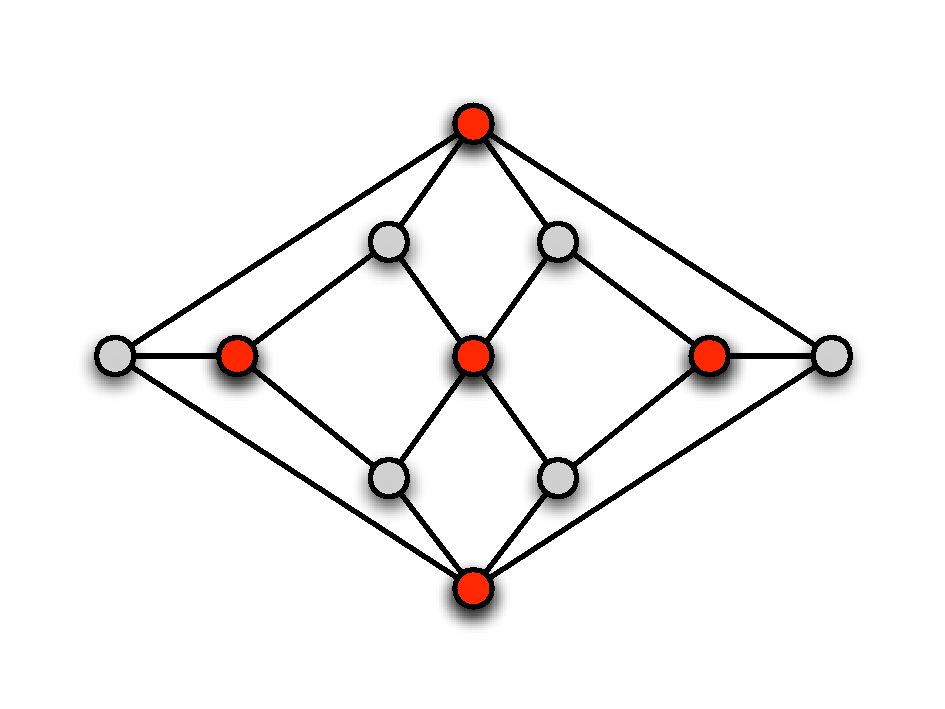
\includegraphics[width=10cm]{pic1.pdf}
\end{center}
\caption{Herschelov graf, vektorska grafika.}
\label{pic1}
\end{figure}
Pa res lahko vključimo slike katerihkoli formatov? 
Žal ne. 
Programski paket \LaTeX\ lahko uporabljamo v več dialektih. 
Ukaz {\tt latex} ne mara vključenih slik v formatu Portable Document Format {\tt .pdf}, ukaz {\tt pdflatex} pa ne prebavi slik v Encapsulated Postscript Formatu {\tt .eps}.
Strnjeno v Tabeli~\ref{tbl:1}.

\begin{table}
\begin{center}
\begin{tabular}{l|ccc}
ukaz/format & {\tt .pdf} & {\tt .eps} & ostali formati \\ \hline
{\tt pdflatex} & da & ne & da \\
{\tt latex}   & ne & da  & da
\end{tabular}
\end{center}
\caption{}
\label{tbl:1}
\end{table}

Nasvet? 
Odločite se za uporabo ukaza {\tt pdflatex}. Vaš izdelek bo brez vmesnih stopenj na voljo v {.pdf} formatu in ga lahko odnesete v vsako tiskarno. 
Če morate na vsak način vključiti sliko, ki jo imate v {\tt .eps} formatu, jo vnaprej pretvorite v alternativni format, denimo {\tt .pdf}.

Včasih se da v okolju za uporabo programskega paketa \LaTeX\ nastaviti na kakšen način bomo prebavljali vhodne dokumente. 
Spustni meni na Sliki~\ref{pic2} odkriva uporabo \LaTeX{}a v njegovi pdf inkarnaciji --- {\tt pdflatex}.
\begin{figure}[t]
\begin{center}
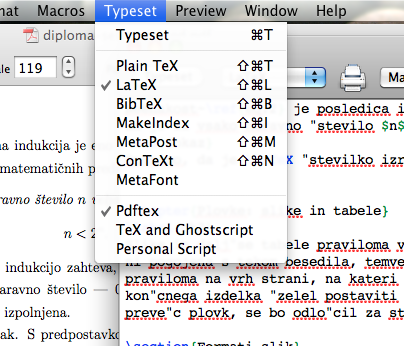
\includegraphics[width=10cm]{pic2.png}
\end{center}
\caption{Kateri dialekt uporabljati?}
\label{pic2}
\end{figure}
Vključena Slika~\ref{pic2} je seveda bitna.



\chapter{Pogoste napake pri pisanju v slovenščini}  % poglavje dodal Solina
\label{slo}

V slovenščini pišemo narekovaje drugače kot v angleščini!   
Običajno uporabljamo dvojne spodnje-zgornje narekovaje:  \sn{slovenski narekovaji}.

Paziti moramo pri uporabi pridevnikov, ki se ne sklanjajo kot so npr. kratice. 
Zato pišemo pravilno model CAD in \textbf{ne} CAD model!

Pika, klicaj in vprašaj so levostični: pred njimi ni presledka, za njimi pa. 
Klicajev in vprašajev se v strokovnih besedilih načeloma izogibajte. Oklepaji so desnostični in zaklepaji levostični (takole).

Pri sklanjanju tujih imen ne uporabljajte vezajev, pravilno je Applov operacijski sistem in \textbf{ne} Apple-ov.

Vezaj  je levo in desno stičen: \verb=slovensko-angleški slovar= in ga pišemo z enim pomišljajem.

V slovenščini je pred in po pomišljaju presledek in ga v LaTeXu pišemo z dvema pomišljajema: \verb=Pozor -- hud pes!=
V angleščini pa je za razliko pomišljaj levo in desno stičen in se v LaTeXu piše s tremi  pomišljaji: \verb=---=.
S stičnim pomišljajem pa lahko nadomeščamo predlog od \dots do, denimo pri navajanju strani, npr. preberite strani 7--11 (\verb=7--11=).



\sn{Pred ki, ko, ker, da, če vejica skače}. To osnovnošolsko pravilo smo v življenju po potrebi uporabljali, dopolnili, morda celo pozabili. 
Pravilo sicer drži, ampak samo če je izpolnjenih kar nekaj pogojev (npr. da so ti vezniki samostojni, enobesedni, ne gre za vrivek itd.).
Povedki so med seboj ločeni z vejicami, razen če so zvezani z in, pa, ter, ne–ne, niti–niti, ali, bodisi, oziroma.
Sicer pa je bolje pisati kratke stavke kot pretirano dolge.


\chapter{Koristni nasveti pri pisanju v \LaTeX{u}}   % poglavje dodal Solina
\label{latex}

Programski paket \LaTeX\ je prvotno predstavljen v priročniku~\cite{lamport} in je v resnici nadgradnja sistema \TeX\ avtorja Donalda Knutha, znanega po denimo, če izpustim njegovo umetnost programiranja, 
Knuth-Bendixovem algoritmu~\cite{knuth1983simple}.

Različnih implementacij \LaTeX{}a je cela vrsta.
Za OS X priporočamo TeXShop, za Windows PC pa MikTeX. Spletna verzija, ki poenostavi sodelovanje pri pisanju, je ShareLaTeX.

Včasih smo si pri pisanju v \LaTeX{}u  pomagali s priročniki, danes pa je enostavneje in hitreje, da ob vsakem problemu za pomoč enostavno povprašate Google, saj je na spletu cela vrsta forumov za pomoč pri \TeX{}iranju.

\LaTeX\ včasih ne zna deliti slovenskih besed, ki vsebujejo črke s strešicami. Če taka beseda štrli preko desnega roba,  \LaTeX{}u pokažemo, kje lahko tako besedo deli takole: \verb=ra\-ču\-nal\-ni\-štvo=.

Predlagamo, da v izvornem besedilu začenjate vsak stavek v novi vrstici, saj \LaTeX\ sam razporeja besede po vrsticah postavljenega besedila. 
Bo pa zato iskanje po izvornem besedilu iskanje in popravljanje veliko hitrejše.

Boljšo preglednost dosežemo tudi z izpuščanjem praznih vrstic za boljšo preglednost strukture izvornega besedila.

S pomočjo  okolja \verb=\begin{comment} ... \end{comment}= lahko  zakomentiramo več vrstic izvornega besedila hkrati.




\chapter{Kaj pa literatura?}
\label{lit}

Kot smo omenili že v uvodu, je pravi način za citiranje literature uporaba \BibTeX{}a~\cite{bib}. 
\BibTeX\ zagotovi, da nobene obvezne informacije pri določeni vrsti literature ne izpustimo in da vse informacije o določeni vrsti vira dosledno navajamo na enak način.

Osnovna ideja \BibTeX{a} je, da vse informacije o literaturi zapisujete v posebno datoteko, v našem primeru je to \texttt{literatura.bib}.
Vsakemu viru v tej datoteki določimo simbolično ime.
V  našem primeru je v tej datoteki nekaj najbolj značilnih vrst literature, kot so knjige~\cite{lamport}, članki v revijah~\cite{leonardo} in zbornikih konferenc~\cite{poglavje_springer}, spletni viri~\cite{bib,video}, 
tehnično poročilo~\cite{andersen2012kinect}, diplome~\cite{diploma} itd.
Po vsaki spremembi pri sklicu na literaturo moramo najprej prevesti izvorno besedilo s prevajalnikom \LaTeX, nato s prevajalnikom  \BibTeX, ki ustvari datoteko  {\tt vzorec\_dip\_Seminar.bbl}, in nato še dvakrat s prevajalnikom  \LaTeX.

Kako natančno se spisek literature nato izpiše (ali po vrstnem redu sklicevanja, ali po abecedi priimkov prvih avtorjev, ali se imena avtorjev pišejo pred priimki itd.) je odvisno od stilske datoteke.
V diplomi bomo uporabili osnovno stilsko datoteko \texttt{plain}.

Z uporabo \BibTeX{a} v slovenščini je še nekaj nedoslednosti, saj so pomožne besede, ki jih \BibTeX\ sam doda,  kot so \textit{editor},  \textit{pages} in besedica  \textit{and} pred zadnjim avtorjem, 
če ima vir več avtorjev~\cite{andersen2012kinect}, zapisane v angleščini,
čeprav smo izbrali opcijo \texttt{slovene} pri paketu \texttt{babel}.
To nedoslednost je možno popraviti z ročnim urejanjem datoteke {\tt vzorec\_dip\_Seminar.bbl}, kar je smiselno šele potem, ko bibliografije v datoteki \texttt{literatura.bib} ne bomo več spreminjali, oziroma ne bomo več dodajali novih sklicev na literaturo
v izvornem besedilu.
Vsebino datoteke {\tt vzorec\_dip\_Seminar.bbl} lahko na koncu urejanja tudi skopirate v izvorno besedilo diplome.

Le če se bomo na določen vir v besedilu tudi sklicevali, se bo pojavil tudi v spisku literature.
V datoteki \texttt{.bib} imamo sicer lahko veliko več virov za literaturo, kot jih bomo uporabili v diplomi.

Vire v \BibTeX\ formatu lahko enostavno poiščemo in prekopiramo iz akademskih portalov za iskanje virov v našo datoteko \texttt{.bib}.
Izvoz v Google učenjaku še dodatno poenostavimo, če v nastavitvah izberemo \BibTeX\ kot želeni format za izvoz navedb.

Pri sklicevanju na literaturo na koncu stavka pazite, da je pika po ukazu \verb=\cite{ }=.
\chapter{Sistem STUDIS in PDF/A}
\label{PDF}

Elektronsko verzijo diplome morate oddati v PDF/A formatu~\cite{pdfa} preko sistema STUDIS.
Natančneje v PDF/A-1b formatu. 

\LaTeX\ in omenjeni format imata še nekaj težav s sobivanjem. 
Paket \texttt{pdfx.sty}, ki naj bi \LaTeX{u} omogočal podporo PDF/A formatu ne deluje v skladu s pričakovanji. 
Ta predloga delno ustreza formatu, vsekakor dovolj, da jo študentski informacijski sistem sprejme. 
Znaten del rešitve je prispeval Damjan Cvetan.

V predlogi, poleg izvornega \texttt{.tex} dokumenta in vloženih slik \texttt{pic1.pdf} in \texttt{pic2.png}, potrebujemo še predlogo datoteke z metapodatki \texttt{pdfa-1b.xmp} in datoteko z barvnim profilom \texttt{sRGBIEC1966-2.1.icm}.




\chapter{Sklepne ugotovitve}

Uporaba \LaTeX{a} in \BibTeX{a} je v okviru Diplomskega seminarja \textbf{obvezna}!
Izbira \LaTeX\ ali ne \LaTeX\ pri pisanju dejanske diplomske naloge pa je pre\-pu\-šče\-na dogovoru med vami in vašim mentorjem.

Res je, da so prvi koraki v \LaTeX{}u težavni. 
Ta dokument naj vam služi kot začetna opora pri hoji.

Vsem raziskovalcem s področja računalništva pa svetujem v branje mnenje L. Fortnowa~\cite{fortnow2009viewpoint}.

\newpage
\ \\
\clearpage
\addcontentsline{toc}{chapter}{Literatura}
\bibliographystyle{plain}
\bibliography{literatura}


\end{document}

